\documentclass[aspectratio=169, table]{beamer}

\usepackage{array}
\usepackage{colortbl}
\usepackage{tabularx}
\usepackage{xcolor}
\usepackage{tikz}
\usetikzlibrary{arrows.meta, positioning, calc, fit, shapes.geometric}

\makeatletter
\def\input@path{{../theme/}}
\makeatother
\graphicspath{{../theme/}{../../figures/}}
\usetheme{Pradita}

\newcommand{\sectionframe}[1]{%
  \begin{frame}{\hfill}
    \centering
    \Huge{\textbf{#1}}
  \end{frame}
}

\newcommand{\takeaway}[1]{%
  \vspace{4pt}
  {\footnotesize #1}
}

\title{\LARGE Governance, Change Management,\\
  \vspace{4pt}
  \& Requirements Management}
\subtitle{IT30713 - Enterprise \& Platform Architecture}
\author{\textbf{Alfa Yohannis}}
\date{1 Agustus 2026}

\begin{document}

\frame{\titlepage}

\begin{frame}[fragile]
  \frametitle{Contents}
  \vspace{20pt}
  \begin{columns}[t]
    \column{0.5\textwidth}
    \tableofcontents[sections={1-4}]

    \column{0.5\textwidth}
    \tableofcontents[sections={5-8}]
  \end{columns}
\end{frame}

\begin{frame}{\hfill}
  \centering
  \Huge{\textbf{Arsitektur target sudah dibangun---bagaimana menjaganya tetap
  benar dan relevan?}}
\end{frame}

% ============================================================
\section{Orientasi Bab}
\sectionframe{Orientasi Bab}

\begin{frame}{Tujuan Pembelajaran}
  \vspace{6pt}
  \begin{itemize}
    \item Menjelaskan \textbf{Implementation Governance} (TOGAF Fase G):
          \emph{Architecture Contract}, \emph{Compliance Review}, \emph{Dispensation}.
    \item Menjelaskan \textbf{Architecture Change Management} (TOGAF Fase H):
          \emph{change driver} \& klasifikasi perubahan.
    \item Menjelaskan \textbf{Requirements Management} sebagai \emph{pusat} ADM:
          \emph{Requirements Repository} \& \emph{traceability}.
    \item Menutup \textbf{siklus ADM}: arsitektur sebagai praktik yang \emph{hidup
          \& terus dikelola}, bukan dokumen sekali jadi.
  \end{itemize}
  \takeaway{Arah sesi: dari ``apa yang dibangun'' menuju ``bagaimana menjaga yang
  dibangun tetap benar \& relevan''.}
\end{frame}

\begin{frame}{Ringkasan Awal Bab}
  \vspace{6pt}
  \begin{itemize}
    \item \textbf{Fase G} memastikan pembangunan \emph{patuh} pada arsitektur
          target (Architecture Contract \& Compliance Review).
    \item \textbf{Fase H} memantau \emph{change driver} lalu memutuskan: governance
          biasa atau \emph{siklus ADM baru}.
    \item \textbf{Requirements Management} menjaga \emph{traceability} dari motivasi
          sampai solusi berjalan---pusat roda ADM.
    \item Studi kasus: menjaga rel Transfer Bank Wanua tetap patuh SNAP BI \&
          teraudit OJK.
  \end{itemize}
  \takeaway{Ini penutup \emph{metode}: menjadikan arsitektur hidup, terkelola, dan
  dapat diaudit.}
\end{frame}

% ============================================================
\section{Roda ADM \& Mekanisme Fase}
\sectionframe{Roda ADM \&\\ Mekanisme Tiap Fase}

\begin{frame}{Roda ADM: Fokus Fase G, H, dan Pusat}
  \vspace{2pt}
  \begin{columns}[c]
    \column{0.46\textwidth}
    \centering
    \scalebox{0.8}{
      \begin{tikzpicture}[
        font=\footnotesize\bfseries,
        phase/.style={circle, draw=praditagreen, line width=0.4mm,
          fill=praditagreen!15, minimum size=11mm, inner sep=0pt},
        hi/.style={circle, draw=blueColor, line width=0.7mm, fill=blueColor!55,
          minimum size=11mm, inner sep=0pt, text=white},
        reqman/.style={circle, draw=orange!80!black, line width=0.6mm,
          fill=orange!30, minimum size=21mm, inner sep=1pt, align=center,
          font=\scriptsize\bfseries},
        prelim/.style={circle, draw=gray!70, line width=0.4mm, fill=gray!18,
          minimum size=13mm, inner sep=0pt, align=center, font=\scriptsize\bfseries},
        ring/.style={-Latex, draw=praditagreen!75, line width=0.4mm},
        spoke/.style={draw=orange!65, line width=0.3mm},
      ]
        \node[reqman] (rm) at (0,0) {Requirements\\Management};
        \foreach \ang/\lab in {90/A, 45/B, 0/C, -45/D, -90/E, -135/F}
          \node[phase] (\lab) at (\ang:2.6cm) {\lab};
        \node[hi] (G) at (180:2.6cm) {G};
        \node[hi] (H) at (135:2.6cm) {H};
        \node[prelim] (P) at (90:4.1cm) {Prelim.};
        \foreach \lab in {A,B,C,D,E,F,G,H} \draw[spoke] (\lab) -- (rm);
        \foreach \a/\b in {A/B, B/C, C/D, D/E, E/F, F/G, G/H, H/A}
          \draw[ring] (\a) to[bend left=12] (\b);
        \draw[ring, draw=gray!70] (P) -- (A);
      \end{tikzpicture}
    }
    \column{0.54\textwidth}
    \footnotesize
    \begin{itemize}\setlength{\itemsep}{1.5pt}
      \item \textbf{\textcolor{blueColor}{G---Implementation Governance}}
            $\leftarrow$ \emph{sesi ini}
      \item \textbf{\textcolor{blueColor}{H---Architecture Change Management}}
            $\leftarrow$ \emph{sesi ini}
      \item \textbf{\textcolor{orange!80!black}{Requirements Management}}---pusat,
            terhubung ke \emph{semua} fase $\leftarrow$ \emph{sesi ini}
      \item A--D---rancangan arsitektur (Sesi 1--7).
      \item E--F---peluang, solusi \& migrasi (Sesi 8).
    \end{itemize}
    \vspace{2pt}
    {\scriptsize Jari-jari oranye = tiap fase memberi \& memakai requirement.}
  \end{columns}
  \takeaway{Bab ini menutup roda: G \& H menjaga arsitektur, Requirements
  Management di pusat menjaga \emph{traceability}.}
\end{frame}

\begin{frame}{Fase G: Lingkar Implementation Governance}
  \vspace{2pt}
  \centering
  \scalebox{0.92}{
    \begin{tikzpicture}[
      font=\footnotesize,
      gov/.style={rectangle, rounded corners=1.5mm, draw=blueColor, fill=blueColor!12,
        thick, align=center, text width=26mm, minimum height=10mm},
      dec/.style={diamond, aspect=2, draw=blueColor, fill=blueColor!6, thick,
        align=center, inner sep=1pt, text width=16mm},
      rels/.style={rectangle, rounded corners=1.5mm, draw=praditagreen,
        fill=praditagreen!15, thick, align=center, text width=22mm, minimum height=9mm},
      flow/.style={-Latex, thick, draw=gray!70}
    ]
      \node[gov] (con) {Architecture\\Contract};
      \node[gov, right=12mm of con] (rev) {Compliance\\Review};
      \node[dec, right=12mm of rev] (d) {Patuh?};
      \node[rels, above right=5mm and 7mm of d] (rel) {Rilis solusi};
      \node[gov, below right=5mm and 7mm of d] (disp) {Dispensation /\\Rework};
      \draw[flow] (con) -- (rev);
      \draw[flow] (rev) -- (d);
      \draw[flow] (d) -- node[above,font=\scriptsize\bfseries]{ya} (rel);
      \draw[flow] (d) -- node[below,font=\scriptsize\bfseries]{tidak} (disp);
      \draw[flow] (disp.west) to[out=180,in=-90] node[left,font=\scriptsize]{tinjau ulang} (rev.south);
    \end{tikzpicture}
  }

  \takeaway{Architecture Contract = \emph{arti patuh}; Compliance Review = gerbang;
  penyimpangan $\rightarrow$ \emph{Dispensation} berbatas waktu atau \emph{rework}.}
\end{frame}

\begin{frame}{Fase H: Mengklasifikasi Perubahan}
  \vspace{2pt}
  \centering
  \scalebox{0.9}{
    \begin{tikzpicture}[
      font=\footnotesize,
      ev/.style={rectangle, rounded corners=1.5mm, draw=purple!60!black, fill=purple!10,
        thick, align=center, text width=26mm, minimum height=10mm},
      cls/.style={rectangle, rounded corners=1.5mm, draw=blueColor, fill=blueColor!10,
        thick, align=center, text width=24mm, minimum height=9mm},
      act/.style={rectangle, rounded corners=1.5mm, draw=praditagreen, fill=praditagreen!14,
        thick, align=center, text width=34mm, minimum height=9mm},
      flow/.style={-Latex, thick, draw=gray!70}
    ]
      \node[ev] (drv) {Change driver\\{\scriptsize teknologi/bisnis/regulasi}};
      \node[cls, right=11mm of drv] (imp) {Nilai dampak \&\\klasifikasikan};
      \node[act, above right=7mm and 11mm of imp] (small) {Simplification / Incremental\\$\rightarrow$ change management};
      \node[act, below right=7mm and 11mm of imp] (big) {Re-architecting\\$\rightarrow$ siklus ADM baru (Fase A)};
      \draw[flow] (drv) -- (imp);
      \draw[flow] (imp) -- (small);
      \draw[flow] (imp) -- (big);
    \end{tikzpicture}
  }

  \takeaway{Tiga kelas perubahan: \emph{Simplification}, \emph{Incremental}
  (governance), \emph{Re-architecting} (memicu ADM baru). Arsitektur tak pernah
  usang tanpa disadari.}
\end{frame}

\begin{frame}{Requirements Management (Pusat ADM)}
  \vspace{2pt}
  \centering
  \scalebox{0.86}{
    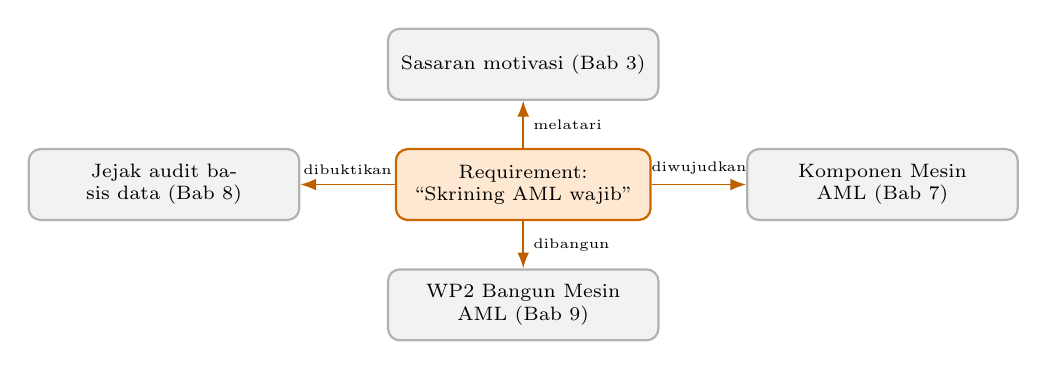
\begin{tikzpicture}[
      font=\scriptsize,
      req/.style={rectangle, rounded corners=1.5mm, draw=orange!80!black, fill=orange!18,
        thick, align=center, text width=30mm, minimum height=9mm},
      lay/.style={rectangle, rounded corners=1.5mm, draw=gray!60, fill=gray!10,
        thick, align=center, text width=32mm, minimum height=9mm},
      link/.style={-Latex, semithick, draw=orange!75!black}
    ]
      \node[req] (r) {Requirement:\\``Skrining AML wajib''};
      \node[lay, above=6mm of r] (mot) {Sasaran motivasi (Bab~3)};
      \node[lay, right=12mm of r] (app) {Komponen Mesin AML (Bab~7)};
      \node[lay, below=6mm of r] (wp) {WP2 Bangun Mesin AML (Bab~9)};
      \node[lay, left=12mm of r] (evd) {Jejak audit basis data (Bab~8)};
      \draw[link] (r) -- node[right,font=\tiny]{melatari} (mot);
      \draw[link] (r) -- node[above,font=\tiny]{diwujudkan} (app);
      \draw[link] (r) -- node[right,font=\tiny]{dibangun} (wp);
      \draw[link] (r) -- node[above,font=\tiny]{dibuktikan} (evd);
    \end{tikzpicture}
  }

  \takeaway{Satu requirement tertaut ke motivasi, komponen, work package, \& bukti
  audit. Inilah yang diminta OJK \& Bank Indonesia.}
\end{frame}

% ============================================================
\section{TOGAF ADM Fase G, H \& Requirements}
\sectionframe{TOGAF ADM Fase G, H \&\\ Requirements Management}

\begin{frame}{Fase G: Input, Langkah, \& Output}
  \vspace{2pt}
  \small
  \begin{columns}[t]
    \column{0.5\textwidth}
    \textbf{\textcolor{praditagreen}{Restoran Go-Online}}
    \begin{itemize}\setlength{\itemsep}{2pt}
      \item \textbf{Input:} Architecture Contract aplikasi pemesanan (keamanan
            pembayaran, integrasi POS \& dapur).
      \item \textbf{Langkah:} bimbing \emph{build} integrasi $\rightarrow$
            Compliance Review pra-peluncuran $\rightarrow$ luncurkan \& review.
      \item \textbf{Output:} Compliance Assessment, Dispensation modul bayar,
            Change Request, aplikasi live.
    \end{itemize}
    \column{0.5\textwidth}
    \textbf{\textcolor{blueColor}{Transfer Bank}}
    \begin{itemize}\setlength{\itemsep}{2pt}
      \item \textbf{Input:} Architecture Contract rel transfer (keamanan gateway,
            batas integrasi core).
      \item \textbf{Langkah:} bimbing \emph{build} gateway/adaptor $\rightarrow$
            Compliance Review WP3 $\rightarrow$ go-live SNAP BI \& review.
      \item \textbf{Output:} Compliance Assessment WP3, Dispensation adaptor core,
            Change Request audit, rel live.
    \end{itemize}
  \end{columns}
  \takeaway{Langkah kanonik: konfirmasi lingkup $\rightarrow$ siapkan sumber daya
  $\rightarrow$ bimbing pembangunan $\rightarrow$ Compliance Review $\rightarrow$
  operasikan \& post-implementation review.}
\end{frame}

\begin{frame}{Fase H: Input, Langkah, \& Output}
  \vspace{2pt}
  \small
  \begin{columns}[t]
    \column{0.5\textwidth}
    \textbf{\textcolor{praditagreen}{Restoran Go-Online}}
    \begin{itemize}\setlength{\itemsep}{2pt}
      \item \textbf{Input:} Change Request (GoFood minta integrasi; usulan ekspansi
            cabang); metrik order.
      \item \textbf{Langkah:} pantau $\rightarrow$ nilai dampak $\rightarrow$
            klasifikasi $\rightarrow$ tangani.
      \item \textbf{Output:} GoFood = \emph{Incremental}; ekspansi multi-cabang =
            \emph{Re-architecting} $\rightarrow$ Request for Architecture Work.
    \end{itemize}
    \column{0.5\textwidth}
    \textbf{\textcolor{blueColor}{Transfer Bank}}
    \begin{itemize}\setlength{\itemsep}{2pt}
      \item \textbf{Input:} Change Request (SNAP BI versi baru; usulan kanal QRIS);
            metrik volume transaksi.
      \item \textbf{Langkah:} pantau $\rightarrow$ nilai dampak $\rightarrow$
            klasifikasi $\rightarrow$ tangani.
      \item \textbf{Output:} SNAP BI = \emph{Incremental}; QRIS =
            \emph{Re-architecting} $\rightarrow$ Request for Architecture Work.
    \end{itemize}
  \end{columns}
  \takeaway{Tiga kelas: \emph{Simplification} \& \emph{Incremental} $\rightarrow$
  change management; \emph{Re-architecting} $\rightarrow$ ADM baru. Aturan: dampak
  $\geq$2 stakeholder $\rightarrow$ cenderung ADM baru.}
\end{frame}

\begin{frame}{RM: Input, Langkah, \& Output}
  \vspace{2pt}
  \small
  \begin{columns}[t]
    \column{0.5\textwidth}
    \textbf{\textcolor{praditagreen}{Restoran Go-Online}}
    \begin{itemize}\setlength{\itemsep}{2pt}
      \item \textbf{Input:} requirement ``estimasi waktu antar akurat'', ``data
            alergi tercatat''; repository.
      \item \textbf{Langkah:} baseline $\rightarrow$ simpan $\rightarrow$ pantau
            $\rightarrow$ Requirements Impact Assessment.
      \item \textbf{Output:} matriks traceability (estimasi $\rightarrow$ mesin
            estimasi $\rightarrow$ log akurasi).
    \end{itemize}
    \column{0.5\textwidth}
    \textbf{\textcolor{blueColor}{Transfer Bank}}
    \begin{itemize}\setlength{\itemsep}{2pt}
      \item \textbf{Input:} requirement ``skrining AML wajib'', ``jejak audit
            lengkap''; repository.
      \item \textbf{Langkah:} baseline $\rightarrow$ simpan $\rightarrow$ pantau
            $\rightarrow$ Requirements Impact Assessment.
      \item \textbf{Output:} matriks traceability AML (kebijakan $\rightarrow$
            Mesin AML $\rightarrow$ WP2 $\rightarrow$ jejak audit).
    \end{itemize}
  \end{columns}
  \takeaway{Di pusat ADM: requirement disimpan di \emph{Architecture Requirements
  Repository}; tiap perubahan dinilai (\emph{Requirements Impact Assessment}) \&
  dijaga \emph{traceability}-nya.}
\end{frame}

\begin{frame}{Contoh Matriks Traceability}
  \vspace{4pt}
  \scriptsize
  {\arrayrulecolor{black!55}\setlength{\arrayrulewidth}{0.3pt}%
  \renewcommand{\arraystretch}{1.3}%
  \begin{tabularx}{\textwidth}{@{}|p{0.185\textwidth}|p{0.15\textwidth}|p{0.155\textwidth}|p{0.075\textwidth}|X|@{}}
    \hline
    \textbf{Requirement} & \textbf{Sasaran} & \textbf{Komponen/Layanan} & \textbf{WP} & \textbf{Bukti/Verifikasi} \\
    \hline
    Skrining AML wajib \emph{(bank)} & Kepatuhan AML \& regulator & Mesin AML \& Limit & WP2 & Jejak audit basis data \\
    \hline
    Transfer real-time \emph{(bank)} & Layanan cepat UMKM & Adaptor BI-FAST & WP3 & Log latensi saat go-live \\
    \hline
    Estimasi antar akurat \emph{(restoran)} & Kepuasan pelanggan & Mesin Estimasi Antar & Online & Log akurasi estimasi \\
    \hline
    Pembayaran online aman \emph{(restoran)} & Kepercayaan pelanggan & Modul Pembayaran & Online & Sertifikasi keamanan kartu \\
    \hline
  \end{tabularx}}

  \takeaway{Tiap \emph{requirement} tertaut satu baris: sasaran $\rightarrow$
  komponen $\rightarrow$ work package $\rightarrow$ bukti---inilah yang ditunjukkan
  ke auditor OJK/BI.}
\end{frame}

% ============================================================
\section{Konsep Inti \& Glosarium}
\sectionframe{Konsep Inti \& Glosarium}

\begin{frame}{Konsep Governance \& Change Management}
  \vspace{4pt}
  \footnotesize
  \begin{itemize}\setlength{\itemsep}{2.5pt}
    \item \textbf{Architecture Contract:} kesepakatan formal yang menetapkan
          \emph{arti patuh}---standar, prinsip, batasan.
    \item \textbf{Compliance Review:} pemeriksaan apakah yang dibangun sesuai
          arsitektur target (gerbang sebelum rilis).
    \item \textbf{Dispensation:} pengecualian \emph{berbatas waktu} atas
          penyimpangan, dengan alasan \& rencana penyelesaian.
    \item \textbf{Change driver:} kejadian yang menuntut penilaian ulang
          arsitektur (regulasi, teknologi, kebutuhan baru).
    \item \textbf{Traceability:} tautan requirement $\rightarrow$ arsitektur
          $\rightarrow$ solusi $\rightarrow$ motivasi.
  \end{itemize}
  \takeaway{Governance = kepatuhan \emph{saat} membangun; change management =
  relevansi \emph{setelah} beroperasi; Requirements Management = benang
  \emph{traceability}.}
\end{frame}

\begin{frame}{Konteks Indonesia}
  \vspace{6pt}
  \begin{itemize}
    \item \textbf{PP 71/2019:} penyelenggara sistem elektronik wajib menjaga
          keandalan, keamanan, jejak, \& melaporkan perubahan signifikan.
    \item \textbf{SNAP BI:} pembaruan standar pembayaran datang sebagai
          \emph{change driver} eksternal yang harus diserap tanpa mengganggu layanan.
    \item \textbf{UU PDP:} setiap perubahan yang menyentuh data nasabah dinilai
          dampaknya sejak awal, bukan setelah insiden.
    \item \textbf{Tata kelola data:} berbagi-pakai data yang terkelola dan
          tertelusur.
  \end{itemize}
  \takeaway{Architecture Contract \& matriks \emph{traceability} = \emph{bukti
  kepatuhan} yang diminta OJK dan Bank Indonesia, bukan formalitas.}
\end{frame}

% ============================================================
\section{Studi Kasus: Restoran \& Rel Transfer}
\sectionframe{Studi Kasus:\\ Restoran Go-Online \&\\ Rel Transfer Bank}

\begin{frame}{Tiga Situasi (Restoran Go-Online)}
  \vspace{4pt}
  \footnotesize
  \begin{itemize}\setlength{\itemsep}{4pt}
    \item \textbf{Situasi 1 (Fase G).} Sebelum peluncuran aplikasi pemesanan
          online, Compliance Review menemukan modul pembayaran belum memenuhi
          standar keamanan kartu $\rightarrow$ \emph{Dispensation} 1 bulan (pakai
          payment gateway pihak ketiga) + Change Request integrasi internal.
    \item \textbf{Situasi 2 (Fase H).} Integrasi ke mitra pengantaran (GoFood)
          $\rightarrow$ \emph{Incremental} (tambah adaptor). Ekspansi banyak cabang
          \& dapur terpusat $\rightarrow$ \emph{Re-architecting} $\rightarrow$
          siklus ADM baru.
    \item \textbf{Situasi 3 (Requirements).} Requirement ``estimasi waktu antar
          akurat'' $\rightarrow$ telusuri: kepuasan pelanggan $\rightarrow$ mesin
          estimasi $\rightarrow$ work package $\rightarrow$ log akurasi.
  \end{itemize}
  \takeaway{Pola G/H/RM sama di domain sederhana (restoran) maupun kompleks
  (perbankan)---berikutnya versi rel transfer bank.}
\end{frame}

\begin{frame}{Tiga Situasi (Rel Transfer Bank)}
  \vspace{4pt}
  \footnotesize
  \begin{itemize}\setlength{\itemsep}{4pt}
    \item \textbf{Situasi 1 (Fase G).} Sebelum go-live SNAP BI, adaptor core
          banking belum berjejak audit penuh. Architecture Board memberi
          \emph{Dispensation} 3 bulan dengan syarat lapisan pencatatan tambahan---
          penyimpangan dikelola, bukan diabaikan.
    \item \textbf{Situasi 2 (Fase H).} BI merilis versi baru SNAP BI: format pesan
          berubah, pola tetap $\rightarrow$ \emph{Incremental} (perbarui contract
          \& adaptor). Usulan kanal QRIS baru $\rightarrow$ \emph{Re-architecting}
          $\rightarrow$ siklus ADM baru.
    \item \textbf{Situasi 3 (Requirements).} OJK meminta bukti kontrol AML $\rightarrow$
          buka matriks traceability: kebijakan $\rightarrow$ komponen $\rightarrow$
          work package $\rightarrow$ bukti audit.
  \end{itemize}
  \takeaway{Governance, change management, dan traceability bekerja bersama menjaga
  rel transfer tetap benar dan patuh.}
\end{frame}

\begin{frame}{Cara Menutup Roda ADM}
  \vspace{4pt}
  \footnotesize
  \begin{itemize}\setlength{\itemsep}{2.5pt}
    \item \textbf{Architecture Contract (G):} arsitektur target menetapkan standar
          yang mengikat tiap work package.
    \item \textbf{Compliance (G):} gerbang Compliance Review sebelum go-live;
          penyimpangan $\rightarrow$ Dispensation/rework.
    \item \textbf{Pemantauan (H):} change driver dinilai \& diklasifikasi.
    \item \textbf{Iterasi (H):} perubahan mendasar memicu ADM baru (kembali ke
          Fase A).
    \item \textbf{Traceability (pusat):} tiap requirement tertaut dari motivasi
          sampai bukti solusi.
  \end{itemize}
  \takeaway{Arsitektur menjadi praktik yang \emph{hidup}: dijaga (G), disesuaikan (H),
  \& ditelusuri (Requirements Management).}
\end{frame}

% ============================================================
\section{Latihan dan Penutup}
\sectionframe{Latihan dan Penutup}

\begin{frame}{Latihan Terapan Individual}
  \vspace{8pt}
  \begin{itemize}
    \item \textbf{Latihan 10.1} -- Architecture Contract \& gerbang Compliance.
    \item \textbf{Latihan 10.2} -- Protokol change management (tiga kelas
          perubahan).
    \item \textbf{Latihan 10.3} -- Matriks traceability (dua requirement kunci).
    \item \textbf{Latihan 10.4} -- Paragraf governance (peran, metrik, regulasi).
  \end{itemize}
  \takeaway{Semua latihan menjadi bahan langsung bagian Tata Kelola, Risiko, \&
  Implikasi Manajerial makalah.}
\end{frame}

\begin{frame}{Penutup: Arsitektur yang Hidup}
  \vspace{6pt}
  \footnotesize
  \begin{itemize}\setlength{\itemsep}{2.0pt}
    \item Tujuh lapisan membangun arsitektur; bab ini menutup \emph{metode}-nya.
    \item \textbf{Governance} (G): yang dibangun setia pada rancangan.
    \item \textbf{Change management} (H): arsitektur menyesuaikan diri dengan
          dunia yang bergerak.
    \item \textbf{Requirements Management:} tiap keputusan dapat ditarik kembali ke
          alasannya.
    \item Menutup roda ADM = merancang arsitektur \emph{dan} cara merawatnya.
  \end{itemize}
  \takeaway{Yang membedakan arsitek enterprise dari sekadar pembuat diagram:
  merancang \emph{dan} menjaga arsitektur tetap hidup, patuh, \& tertelusur.}
\end{frame}

\begin{frame}{\hfill}
  \centering
  \Huge{\textbf{Terima kasih}}\\[8pt]
  \normalsize Pertanyaan \& diskusi
\end{frame}

\end{document}
